% ====================================================================

\documentclass[psfig,11pt]{article}
\usepackage{graphicx}
\setlength{\textheight}{9in}
\setlength{\topmargin}{0in}
\setlength{\baselineskip}{0.1in}
\setlength{\textwidth}{6.3in}
\setlength{\oddsidemargin}{0in}
\def\cf{{\it cf.}}
\def\eg{{\it e.g.}}
\def\ie{{\it i.e.}}
\def\etal{{\it et al.}}
\def\etc{{\it etc}}
\def\ni{\noindent}
\def\go{\mathrel{\raise.3ex\hbox{$>$}\mkern-14mu\lower0.6ex\hbox{$\sim$}}}
\def\lo{\mathrel{\raise.3ex\hbox{$<$}\mkern-14mu\lower0.6ex\hbox{$\sim$}}}

% ====================================================================

\begin{document}

\section*{PROJECT DESCRIPTION}

% --------------------------------------------------------------------

\section{Introduction}

\subsection{Mapping our Universe}

The earliest examples of astronomy included following the nearby planets and charting the ``fixed'' stars which were projected onto the celestial sphere and organized into constellations. Ultimately this led to a physics-based, low resolution,  3D description of the Galaxy. The situation today in cosmology is somewhat similar. We have large surveys of comparatively nearby galaxies and a splendid two dimensional map of the microwave background and this has led to a standard model of the universe in which inflation-based, Gaussian, potential fluctuations, with a well-defined spectrum, grew according to deterministic laws to produce contemporary large scale structure in a flat universe that is endowed with a cosmological constant. However, the traditional goal of astronomy, to describe the complete disposition of this actual structure, has hitherto been subsumed into statistical investigations designed to elucidate the underlying physics.

This is a staged proposal to combine recent observations with what we have learned about the physics to make the best map we can of the 3D structure of the universe within and slightly beyond our horizon. In addition to satisfying a natural desire to describe our universe, success in this program will naturally furnish ongoing and planned investigations with additional priors which should tighten up their accuracy.

\subsection{Contents}

The last decade has seen remarkable advances in cosmology, spearheaded by increasingly detailed measurements of the cosmic microwave background (CMB) radiation (Adam et al. 2015). These accurate measurements have affirmed that a description of a homogeneous, spatially flat general relativistic universe with relatively few ingredients -- photons ($T_\gamma=2.7$~K), neutrinos (three flavors), baryons ($\Omega_b=0.05$), dark matter ($\Omega_d=0.26$) and a cosmological constant ($\Omega_\Lambda=0.69$) supplemented by (almost) scale-free, adiabatic, Gaussian initial perturbations suffices to describe essentially all that is secure in the observations. There is still room for revision, retractions and new discoveries but, right now, we have a good working hypothesis that the universe is basically this simple (e.g. Weinberg 2008, Schneider 2015). There is some tension in the reported measurements of the Hubble constant (68 ~km s$^{-1}$ Mpc$^{-1}$) etc but this is not important for our purpose and we shall simply adopt Planck values. Much effort is being expended to see if a ubiquitous and eternal cosmological constant needs to be replaced by a dynamical dark energy. If this turns out to be true then simple changes will be needed to what follows.

\subsection{Evolution}

The description of the average expansion of the universe is relatively uncontroversial. When  $t\sim 50$~kyr,  the scale factor -- the size of a region relative to its contemporary size -- was $a\sim0.0003$ and the universe became (dark) matter-dominated. When $t\sim380$~kyr, $a\sim0.0009$, the hydrogen plasma quickly formed atoms, decoupling from the radiation and forming the inside-out, CMB photosphere where the majority of CMB photons we observe today were last scattered with a temperature $\sim2900$~K. When $t\sim600$~Myr, $a\sim0.1$, the first stars formed and the universe (re)-ionized. This epoch is becoming accessible to observation. Finally when $t\sim8$~Gyr, $a\sim0.6$, the cosmological constant came to dominate over the matter, and the universal expansion started to accelerate.

\subsection{Fluctuations}

The observed fluctuations are conventionally described by a set of spatial Fourier modes expressed in terms of contemporary or comoving coordinates. These modes are longitudinal and the ones that mostly concern us here evolved linearly. It is convenient to describe their amplitude using the (effective) Newtonian potential $\Phi$,\footnote{It is simplest to work in the ``Newtonian'' gauge throughout.} from which the density and fluid velocity perturbations can be simply computed. The radiation and neutrinos have to be treated kinetically and a second scalar curvature potential needs to be introduced for accurate calculations. There may also be tensor modes which we shall ignore here. If, and when, they are detected, only minor modifications will be needed. The modes that mostly concern us remain linear and are ``adiabatic'', so that we only need to know their amplitude and phase at one epoch, e.g. recombination, to predict them for all time.

It has recently been demonstrated, mainly using CMB observations, that the adiabatic hypothesis is quite accurate. Furthermore, the amplitudes associated with each mode of the initial potential scale as $k^{-3/2}$ and are drawn from a Gaussian distribution, so that the potential fluctuations associated with each length scale are scale-independent.\footnote{Actually there is a small tilt in their power spectrum in the sense of there being slightly larger amplitudes at longer wavelengths. This requires a small correction to what follows.} This behavior is consistent with a remarkable early conjecture by Harrison (1970) as elaborated by Zel'dovich (1972). 

The potential associated with a mode was essentially frozen until it ``entered the horizon,'' that is, until the timescale for its dynamical evolution, $a/k$, became smaller than the Hubble timescale (which can be thought of as the estimated age of the Universe if the expansion rate were constant).
%until its wavelength became smaller than the Hubble radius. If
   We are mostly concerned with wavelength modes for which this happened before recombination and $k<k_0\sim40{\rm Gpc}^{-1}$.\footnote{$k_0$ can be considered as approximately the wavenumber associated with the first acoustic peak and its consequence, Baryon Acoustic Oscillations (BAO).} For such wavenumbers, the waves evolve at roughly constant $\Phi$ until the cosmological constant takes over and the potential falls by roughly 20 percent today. We make this explicit in Fig.~1 where we show the interior of the last scattering surface in comoving coordinate space and a particular wave whose amplitude and phase we are trying to measure.
\begin{figure}[t]
\centering
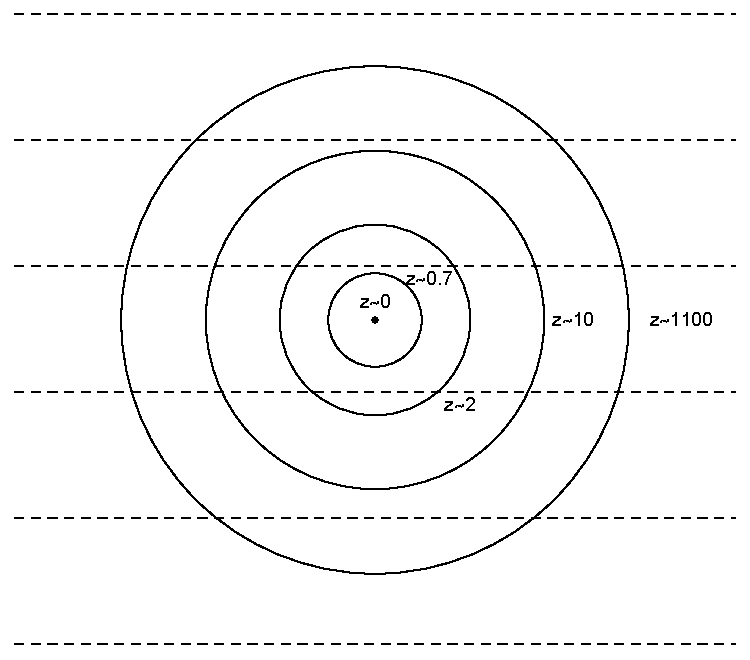
\includegraphics{nsffig.pdf}
\caption{The local universe interior to the CMB photosphere expressed in comoving coordinates. The circles are, in order, redshift $z\sim0.7$, schematically the limit of present surveys, $z\sim2$ roughly the effective limit of future surveys, the nominal Epoch of Reionization at $z\sim10$ and the CMB photosphere at $z\sim1100$ and a distance $x_{\rm CMB}\sim14$~Gpc. Also shown as dashed lines are the nodes of a single wave mode with $k\sim0.4$~Gpc$^{-1}$ which contributes significantly to spherical harmonics up to $\ell\sim6$. The universe that is directly observable by us (for example using long wavelength gravitational waves) extends only slightly beyond the CMB photosphere. WILL REDRAW AND SHRINK.}
\end{figure}

\subsection{Inflation}

The flatness of the geometry today, the isotropy of the CMB temperature, and the very existence of fluctuations with wavelengths longer than naively allowed by causality are all consistent with the simplest version of a much more specific and even bolder conjecture by Guth(1981), Linde(1982) and others, that the universe underwent a period of so-called ``inflation'' at much earlier times. This theory is based on the idea that all the structures in the observed universe emerged from quantum fluctuations about $10^{-33}$ seconds after the Big Bang. Inflation, which describes a phase of accelerated cosmic expansion, is the leading theory providing a causal mechanism for generating these fluctuations and stretching them to cosmological scales. The microphysics of inflation makes detailed predictions for the spectra of these fluctuations as observed in the CMB, in particular their slightly tilted power spectrum.

Qualitatively, the causal mechanism seeding the primordial perturbations is easily understood. During inflation, the Hubble radius, $H^{-1}$, which can be thought of as the ``apparent horizon", remains (quasi) constant. Meanwhile, quantum fluctuations in the matter field(s) and metric are constantly generated with wavelength $H ^{-1}$ at most. Once produced, a fluctuation with comoving wavelength $\lambda$ is stretched with the expansion of space past the Hubble radius, at which point its dynamical timescale, $a/k$, becomes larger than the Hubble time, it ``exits the horizon'', and its amplitude freezes.  Throughout inflation, such fluctuations are continuously created on the physical scale $H^{-1}$. Therefore, by the end of inflation, perturbations will finally have been produced on a whole spectrum of physical scales.


%We do not understand the underlying physics, but the general outcomes of this mechanism have been corroborated wherever this is possible. 

\section{Proposed Research}

\subsection{Long-term Goal}

The long term goal which this proposal addresses, is to connect the CMB to local surveys, and to produce an evolving three-dimensional (or in other words, a 4D) map of the universe that is valid from before 380~kyr to today, and out beyond 14 Gpc. The exercise is not purely cartographic as it is essential that we use the secure physical inferences that have been drawn about the early universe in making this map.

The first stage of our proposed program uses 2D Cosmic Microwave Background (CMB) observations alone to test internal consistency and to recover as much as we can of the 3D potential, velocity and density fields interior to the last scattering surface. In the second stage, we augment CMB data with existing 3D measurements from galaxy surveys, gravitational lensing, intermediate Sachs-Wolfe measurements and so on. This should improve the resolution. The third stage involves estimating the improvement that should come on a decade timescale from future surveys such as LSST and Epoch of Reionization investigations, ``Stage IV'' CMB observations, SKA etc. The fourth and final stage is an investigation of how far it is possible to reconstruct the structure of the universe including what can be inferred beyond our horizon.

% - - - - - - - - - - - - - - - - - - - - - - - - - - - - - - - - - -

\subsection{Stage 1. From 2D to 3D: Gravitational Potential Reconstruction from CMB Surface Data}

\subsubsection{CMB temperature fluctuations}

Most quantitative cosmology derives from CMB observations. The conventional way to describe the observations is in terms of spherical harmonics -- the generalization of Fourier modes to a sphere -- labeled by $\ell$ and $m$. It is convenient to use an equivalent vector of real spherical harmonics, $Y_y(\theta,\phi)=\{Y_{0,0},Y_{1,0},2^{1/2}\Re[Y_{1,1}],2^{1/2}\Im[Y_{1,1}],Y_{2,0},\dots,2^{1/2}\Im[Y_{\ell_{\rm max},\ell_{\rm max}}]\}$ of length $(\ell_{\rm max}+1)^2$ and where $\theta,\phi$ are standard spherical polar coordinates. Note that there are $2\ell+1$ independent, real, basis function in each $\ell$-shell. Note also that $\int d\Omega Y_yY_{y'}=\delta_{yy'}$. It is convenient to treat $\ell_{\rm max}$ as a continuous variable by adding a fraction between zero and unity of the largest $\ell$ shell and therefore smoothly change the angular resolution.
\begin{figure}[t]
\centering
%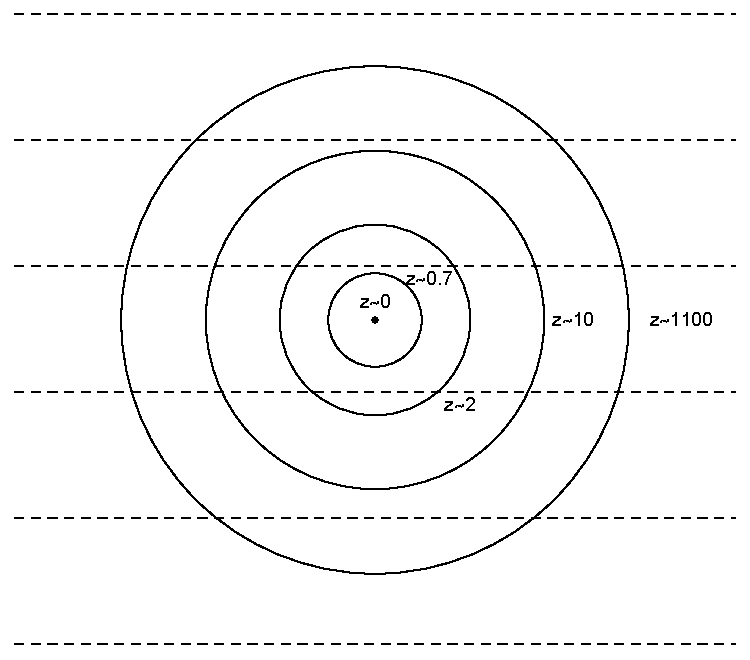
\includegraphics{nsffig.pdf}
\caption{Photospheric potential fluctuations of the CMB for $\ell=2,4.5,10$ derived from Planck data shown as Mollweide projections.}
\end{figure}

Most investigations have focused on measuring the ``power'' in the temperature fluctuations (including polarization) associated with a given $\ell$, obtained by summing products of the coefficients of the harmonic components over $m$, and comparing it with the predictions of various cosmological models. This program has been wonderfully productive, and has resulted in the world model just outlined. Furthermore this power spectrum has been successfully reconciled with features of the local universe, such as galaxy counts. One common assumption is that the particular realization of the universe that we are observing is drawn from a statistical ensemble of universes. When $\ell$ is large, we have many independent measurements on the associated angular scale, $\sim\pi/\ell$, and so we can measure an rms value for the harmonic component with a small variance. However, when $\ell$ is small, we have only a few such measurements and the ``cosmic'' variance is large. Despite their great value, these statistical measurements inevitably discard information which may be valuable.\footnote{This is in the sense that music is far more than a ``flicker'' power spectrum. To pursue our musical metaphor, different voices and instruments contribute different ranges of frequencies to a musical performance over a total range of roughly ten octaves. We are only listening to the bass range but higher voices and instruments can still contribute to what we hear.}  In the proposed study, only one specific realization of the universe -- the one we inhabit --  is considered.

In order to start us on a pilot investigation, the Planck team (IDENTIFY INGE OR NOT?) has kindly supplied us with 100 realizations of Planck temperature fluctuation data for $0\le\ell\le10$ or $1\le y\le121$. From this we are able to compute the mean photospheric potential fluctuation maps at the time of recombination $\Phi=a_yY_y$, (including the monopole and dipole components and adopting the summation convention) and the covariance matrix $C_{yy'}$ associated with the harmonic components $a_y$. We find that this matrix is invertible and can be used directly up to $\ell=8$. More careful treatment of the data is needed beyond this. The fractional variance in individual harmonics varies between $\sim0.0001$ and $\sim0.01$. Undoubtedly there are systematic effects present in this data set which need to be explored but the accuracy is high enough to proceed without this.

\subsubsection{Fourier Modes}
It is conventional to Fourier expand the potential $\Phi$ at a given time, usually the present; the expansion at other times is then simply calculable. Although the full spectrum of the Fourier modes we are discussing is continuous in ${\bf k}$, the fact that our observations are made over a restricted volume means that we can treat the waves as a discrete Fourier transform of modes associated with a box in comoving space of side $L$ on which periodic boundary conditions are imposed. $L$ is chosen here to have a compromise value of four times the radius of the cosmic photosphere, $13.9$~Gpc\footnote{The comoving radius of the big bang is $14.2$~Gpc.} which we adopt as our unit of length.
\begin{equation}
\Phi[{\bf x}(x,\theta,\phi)]=\sum_{n=1}^{N/2}[f_n\cos({\bf k}_n\cdot{\bf x})+f_{N+1-n}\sin({\bf k}_n\cdot{\bf x})]
\end{equation}
where the coefficients $f_n$ are real and ${\bf k}=\Delta k\{n_1,n_2,n_3\}$, with $n_1,n_2,n_3$ integers and $\Delta k=2\pi/L=\pi/2$.  We restrict the sum to $(n_1^2+n_2^2+n_3^2)^{1/2}\le n_{\rm max}$ and only need consider $\bf k$ over a hemisphere. We label the coefficients by the index $n$ running from $1$ to $N\sim4\pi n_{\rm max}^3/3$. ($N=6$ through $4168$ for $n_{\rm max}=1$ through $10$.) $\Phi({\bf x})$ can be expanded formally as an infinite sum of Legendre polynomials and approximately as a finite sum:
\begin{equation}
\Phi({\bf x;\ell})=\sum_{\ell'=0} ^\ell(2\ell'+1)\sum_{n=1}^{N/2}j_{\ell'}(k_nx)P_{\ell'}({\hat{\bf k}}_n\cdot{\hat{\bf x}}[\cos(\ell\pi/2)f_n+\sin(\ell\pi/2)f_{N+1-n}].
\end{equation}

\subsubsection{Gaussian Prior}
Detailed study of the CMB has led to the conclusion that the amplitude of each discrete mode with wave vector $\bf k$ is drawn from a Gaussian distribution of variance $\sigma_n^2=A(n_1^2+n_2^2+n_3^2)^{-3/2}$. We determine the coefficient $A$ by first expressing the spherical harmonic coefficients $a_y$ in terms of the Fourier coefficients according to:
\begin{equation}
a_y=R_{yn}f_n, {\rm where}\ R_{yn}=4\pi Y_y(\theta'\phi')j_\ell(k)[\cos(\pi\ell/2),\sin(\pi\ell/2)]\ {\rm for}\ [1\le n\le N/2,N/2<n\le N],
\end{equation}
and fitting the mean measured spherical harmonics to this relation. We find that $A=????$. (This is adequate for our pilot study, but an improved determination using the evidence follows the approach of Suyu et al. 2006.)
\subsubsection{Preliminary Results}
The simple question that motivated this investigation, and which did not seem to have a well-known answer, was how much of the 3D potential could be reconstructed interior to the 2D CMB photosphere using CMB observations alone. This is an example of what is sometimes called holography.\footnote{This is not the original meaning of the word.}  At first sight this might seem hopeless, because if one associates $\ell$ with $kx_{\rm CMB}$, then we are trying to solve for $O((k_{max}r_{\rm CMB})^3)$ Fourier modes using only $O(\ell_{max}^2)$ spherical harmonics. However, if we confine our attention to the longest wavelength waves, use all the information that is at our disposal exploit the high accuracy of the measurements while accepting uncertainty in the result, then it is possible to make some progress.

We do this by estimating the coefficients $f_n$ through maximizing the likelihood or, equivalently, minimizing the quantity 
\begin{equation}
-2\ln{\cal P}=(a_y-R_{yn}f_n)C_{yy'}^{-1}(a_{y'}-R_{y'n}f_n)+\frac{f_n^2}{\sigma_n^2}
\end{equation}
where $C_{yy'}^{-1}$ is the inverse of the covariance matrix, with respect to $f_n$. This leads to the linear equations:
\begin{equation}
f_n=\left(\sigma_n^{-2}+C_{yy'}^{-1}R_{yn}R_{y'n}\right)^{-1}R_{yn}C_{yy'}^{-1}a_{y'}
\end{equation}

So far, we have tested this procedure using fake data and found that it is generally possible to recover low order Fourier coefficients. We have also used the actual Planck data and our results are exhibited in Fig.~3. 
\begin{figure}[t]
\centering
%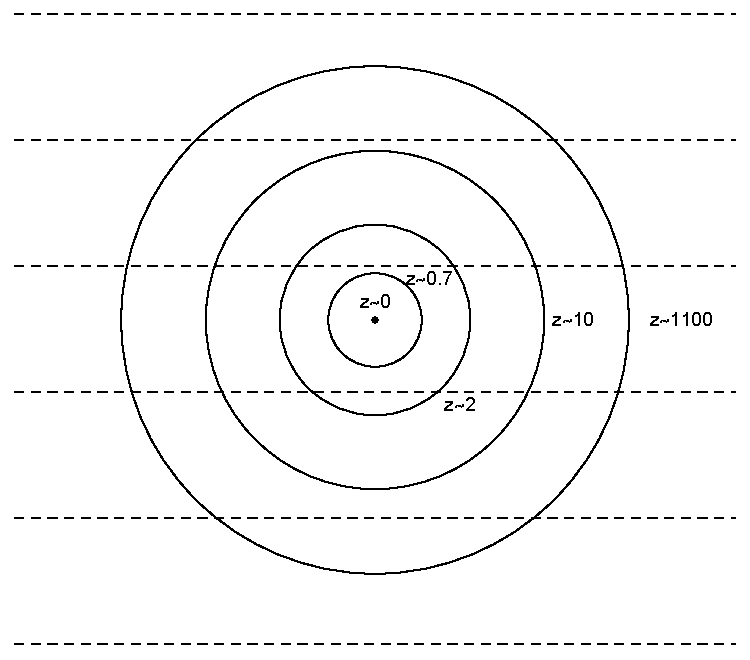
\includegraphics{nsffig.pdf}
\caption{Preliminary recovery of the potential $\Phi$ at the time of inflation from the CMB data alone. Fourier coefficients up to $n_{\rm max}=???$ are used. A higher resolution map should be possible using a more sophisticated inversion process and including polarization data.}
\end{figure}
\subsubsection{Inflationary Origin of Observed Perturbations and Hyperparameter Estimation}

LAURENCE TO DRAFT UP TO 1PAGE INCLUDING FIGURE


\subsubsection{Detailed Approach Incorporating Planck Polarization DATA}

PHIL AND LAURENCE TO DRAFT UP TO 1PAGE


\subsubsection{Tree Representation and Non-Parametric Investigation of Gaussianity}

ROGER TO DRAFT AND SHOW FIRST SURFACE RESULTS

There is another way to think about this problem. Smooth the potential as defined on the last scattering sphere by convolution or restricting the number of spherical harmonics that are included. Consider the zeros of its 2D gradient which will be isolated maxima, minima and saddle points. Next consider the equipotentials that pass through the saddles - called separatrices - which define a nested set of contours. Now imagine these contours being extended as nested surfaces within the sphere. In addition, continue the zeros as lines inside the sphere. These lines meet at points where the 3D gradient vanishes. The organization and nesting of these points, lines and surfaces defines a specific topology.

However, without additional rules, any solution that respected the topology would be as good as any other.\footnote{One thing that can be said is that the fraction of zeros on the sphere that are saddles can be computed for a given prior on the potential Fourier components and this may provide another way to limit non-Gaussianity. Another comment is that this set up provides a natural and possibly fruitful use for the Gauss-Bonnet theorem (e.g. Carroll 2004).} For example, if the potential had satisfied a specific partial differential equation such as  Laplace's equation, then the interior solution could have been completely specified by the surface (Dirichlet) conditions. Our invocation of Gaussian priors on the Fourier modes and imposition of the maximum likelihood prescription leads to a specific solution but our confidence in it diminishes as the number of zeros increases or, equivalently, the angular resolution decreases. Finding the optimal way to carry this out in practice, including the polarization data and the results of local surveys, is a major inference problem and this is what this proposal is really about.

At the time of writing, this investigation is still underway but so far, the results are encouraging. As long as the spherical harmonic coefficients are measured relatively accurately, hundreds of Fourier components can be recovered. We propose to continue this investigation and if this finding is confirmed to understand in much more detail this well-posed, albeit somewhat artificial, problem. In particular, we need to understand  the optimal number of Fourier components and spherical harmonics to include in the reconstruction for a given CMB map accuracy.

The next step will be to carry out an investigation using simulated temperature data as measured at points on the sky, and finding the optimal procedure to recover the body modes directly from the raw data not from derived quantities where additional complications may arise. Finally, the actual Planck data will be used and the results compared with the simulations if appropriate. The accompanying covariance matrix will indicate how well the underlying assumptions are satisfied, while the posterior predictive residual maps will reveal how well the systematic effects inherent in CMB data have been handled. If the initial indications are realistic then a linear resolution of order 1.5~Gpc should be attainable.

\subsubsection{Surface Modes}

The above procedure will work at most for long wavelength body modes. There are three reasons why it must fail for short wavelength modes: there are too many to recover, their amplitudes are small and the CMB photosphere actually has a finite width  $\sim0.1$~Gpc dictated by the actual rate at which the hydrogen recombined. The radiative transfer through the last scattering shell is essential for relating the CMB polarization data to the total temperature fluctuations. It is possible, in principle, to predict the polarization given the temperature fluctuations, and this exercise is likely to be carried out in the next Planck data release. It will also be re-examined in the context of the proposed investigation as it provides an important check on the underlying assumptions.

This suggests an alternative approach to deriving the interior potential map, and this is to use the existing data to continue the potential relatively close to the last scattering surface as has previously been proposed by Yadav \& Wandelt (2005) who also considered recovering longer wavelength modes. This approach will work best around the acoustic peak $\ell\sim200$ and somewhat shorter, where the wavelengths are comparable with the shell thickness. In this calculation the goal will be to recover local Fourier modes by flattening the last scattering surface. We propose to carry put this exercise too using public data and to reconcile this approach with the body wave reconstruction. It will also teach us how to handle maps where, somewhat unusually, our ability to see detail improves with distance.

An important part of this process is to understand the detailed evolution of the individual Fourier modes through recombination. Although, perfectly adequate and publicly available packages have been developed to carry this out, they seem to lack physical transparency which we will need and so an alternative Monte Carlo approach is under development to help elucidate more clearly how the evolution of a individual mode is expressed as a CMB fluctuation.

% - - - - - - - - - - - - - - - - - - - - - - - - - - - - - - - - - -

\subsection{Stage 2. From 3D to 4D: Incorporating Existing Volumetric Data}

\subsubsection{CMB Lensing and ISW measurements}

An important way to add 3D information is to include CMB lensing (Ade et al. 2014b). A uniform CMB is unchanged by gravitational lensing. However, if there is a gradient in the background temperature, intervening structure will appear as extra power on the scale of intervening large scale structure.\footnote{More subtle manifestations including those involving polarization are possible (Hu \& Okamoto 2002), but this is the main effect.} The consequences are largest on much smaller scales than those in which we are primarily interested. However there are still integral effects with $\ell\sim30-100$ which are relevant. Furthermore the intense interest in the claim that inflationary B-modes have been detected (Ade et. 2014c)  has focused much observational and analytical effort on this region of the spectrum. It is proposed to see if the addition of these measurements will improve the specification of the 3D body modes.

Similar remarks apply to the Integrated Sachs Wolfe effect which is caused by changes in the potential due to the cosmological constant at late times. It is proposed to see if such measurements can also contribute to the specification of large scale structure although here the challenge seems even greater.

\subsubsection{Galaxy Surveys and the Local Universe}

Most of the use of surveys has been for drawing statistical inferences relating the growth of structure to the CMB emphasizing shorter length scales, notably those associated with BAO and the largest voids $\sim0.1$~Gpc. However, these same surveys can also be used to augment the long wavelength CMB data and improve the accuracy and resolution of the resulting 3D map. A good example is the SDSS/BOSS program http://www.sdss.org which covered nearly a third of the sky with over a million redshifts and photometry on galaxies out to $z\sim0.7$.\footnote{21 cm redshift surveys provide an important complement to optical surveys but the survey volumes to date are comparatively modest.} For our purposes this translates to a comoving volume $\sim50{\rm Gpc}^3$, about 0.005 of the total. Surveys of much rarer quasars and the brightest star forming galaxies which extend to  $z\sim6$ provide much greater volumes over which the potential on Gpc scales can be estimated but with inferior precision.

It is helpful at this point to consider a volume limited-survey of objects out to some radius $r$. Suppose we have a set of objects, ($L^\ast$ galaxies, quasars, bright, star-forming galaxies $\dots$) with space density $n$ and we want to measure the amplitude of a given Fourier component with wave vector $k$ of the relative density perturbation associated with this potential $\delta\sim-2k^2\Phi/3a^2H^2$. Now the precision with which the amplitude of a single relative density perturbation Fourier mode can be measured is comparable with the precision with which the fractional density perturbation can be measured in a single region of size equal to the associated length scale. This is $\sim k^{3/2}n^{-1/2}$ and must exceed $\delta$. This suggests that the density of such objects must exceed $\sim H_0^4/c^2\Phi k_max$ if local surveys can possible connect with the CMB. A slightly more careful calculation indicates that making such a connection with existing survey and CMB data from stage 1 is just possible and so it is worth exploring this further. If, this is achievable, then although the data increment will be small, its value will be much greater because it can act as a phase reference for anchoring the imperfectly specified modes measured by CMB observations.

% - - - - - - - - - - - - - - - - - - - - - - - - - - - - - - - - - -

\subsection{Stage 3. Future Surveys}

\subsubsection{Ground-based CMB Telescopes}

PHIL TO REVISE THIS SECTION

While there are exciting proposals for future space-based CMB measurements, most attention is currently focused on the next two generations - Stages 3 and 4 - of ground-based CMB telescopes proposed to deliver results in very roughly five and ten years respectively. While these are mostly focused on probing the physics of inflation and neutrinos, they will also improve the measurement of temperature and E-mode polarization on the scales $\ell\lo200$ in which we are primarily interested with signal to noise $\sim3\times10^{-4}$, roughly ten times better than Planck.

\subsubsection{Survey Telescopes}

Construction has begun on the Large Synoptic Survey Telescope (LSST) http://www.lsst.org/lsst/ which will commence a decade-long survey in 2022. It will survey half the sky (with very strong overlap with the ground-based CMB observations) in six bands detecting about ten billion galaxies out to $z\sim2$ for $L^\ast$ galaxies and $z\sim6$ for bright, star-forming galaxies and quasars. Its primary cosmological goal is to perform a weak lensing survey to see if dark energy (and not just a cosmological constant) is responsible for cosmic acceleration, but it will, in reality, contribute to many more important cosmological measurements. LSST will only provide photometric redshifts, well-calibrated by large spectroscopic surveys such as DESI http://desi.lbl.gov which is projected to measure $\sim20$ million redshifts to $z\sim1$ starting in 2018. As with the CMB, optical weak lensing observations can provide ``tomographic'' distance information and, in principle, should lead to a better map of the long wavelength perturbations. Another source of new local data will be the Euclid space mission http://www.euclid-ec.org which is scheduled for a 2020 launch and which will carry out weak lensing, baryon acoustic oscillation and redshift space distortion measurements using 1.5 billion galaxies and 50 million redshifts over more than a third of the sky. The proposed WFIRST-AFTA http://wfirst.gsfc.nasa.gov also has an impressive program in observational cosmology. At radio wavelengths, the Canadian High Intensity Mapping Experiment (CHIME) http://chime.phas.ubc.ca will measure BAO out to $z\sim2.5$ over half the sky.

\subsubsection{Epoch of Reionization}

There is a large effort underway to probe the Epoch of Reionization, {EoR) $6\lo z\lo30$ through hydrogen line measurements. This is an exciting area of discovery as the relevant physics depends upon many factors, notably first star formation and galaxy assembly that are very hard to anticipate.\footnote{JWST, http://www.jwst.nasa.gov scheduled for launch in 2018, will also help indirectly in understanding the universe during this epoch but seems unlikely to provide quantitative measurements of very large scale structure.} The experiments will probe an ideal range of comoving radius $\sim8-12$~Gpc, interpolating between the CMB photosphere and local surveys,  for either contributing to or expanding upon our incorporating our 3D potential map.

On a longer time scale there are ambitious plans to construct an international Square Kilometer Array (SKA) https://www.skatelescope.org. The long term goals include measuring the redshifts of a billion galaxies, performing weak lensing surveys and carrying out more sensitive surveys of the epoch of reionization. It is likely that the SKA capabilities and schedule will become better-defined over the lifetime of this proposed research program.

\subsection{Stage 4. Future Possibilities}

\subsubsection{Limits to Mapping}

Although it is proposed to examine the possible roles of many new facilities, it is of interest to consider the limitations to what could be learned about the idiosyncratic structure of our local universe on cosmological length scales with {\it any} conceivable observing facility operating for say a generational time (cf. Leclerc et al. 2014). This is mostly a question of spatial resolution though it is also partly a question of signal to noise.\footnote{An interesting analogy is the measurement of helioseismic modes where the basic spectroscopic job is largely complete and research interest has moved on to understanding the physics of the excitation and damping of the modes.} This cosmic uncertainty principle might be expressible in terms of quite basic principles.

\subsubsection{Fundamental Physics and Cosmology}

Although this proposal began by making a clear distinction between the physics-driven research largely executed through statistical measurements and mapping our cosmological neighborhood out to $\sim15$~Gpc, it is pretty clear that, if it is successful, then the maps may actually be able to contribute to answering more fundamental questions. Here we list a few quick and relatively obvious issues to consider. It should be possible to explore space significantly outside our horizon using the inferred low frequency modes. In practice this will only amount to saying that something egregious - a colliding bubble or brane - has not happened close enough to our past light cone to have crossed it. This might possibly be of interest for some versions the landscape that conclude that the actually number of inflationary e-foldings that happened has to be very close to the minimum required.  Another possible benefit is that knowing the gravitational potential allows one to predict the average bulk doppler shift and gravitational redshift that may be measurable for example using observations of Type 1a supernovae. More generally, both the CMB and the survey data, should be improved by insisting on agreement between them. More accurate cosmological parameters should ensue, because we are not doing two separate marginalizations over the phase information at each epoch. Another reward should be helping to handle the vexacious problem of bias by being able to specify the underlying density field. This will, in turn, improve many cosmological tests.

Undoubtedly, the truly ambitious goal for this program which would be transformative, would be to connect individual modes around the first acoustic peak where their amplitude is statistically large, to the corresponding BAO modes measured in large redshift surveys. This would greatly improve both the accuracy (not just the precision) with which cosmological parameters can be measured because it is essentially kinematic and the k's can be calculated for a given set of basic parameters and do not have to be calibrated astronomically. As of this writing, the goal seems out of reach but the possibility is certainly worth further consideration.

% ====================================================================

\section{Personnel Plans}

This work will be primarily a collaboration between the PI and the co-Investigator Dr.\ Phil Marshall who is currently a Project Scientist at SLAC and chair of the LSST Dark Energy Science Collaboration Council. It is proposed to support a postdoctoral fellow to work on this project one third time. Ideally we would like to employ the same person for all three years as continuity will be very helpful in achieving the long term goals. Other factors being equal, we will give preference to someone who also has an interest in the public outreach aspects of this program.

Several other colleagues at KIPAC, notably Sarah Church, Ryan Keisler and Bob Wagoner have expressed interest in this project and will act as consultants and possibly collaborators on the research.

% ====================================================================

\section{Responsibilities and Schedule}

Blandford will start by taking the lead experimenting with the simulation of potential maps and then CMB temperature and polarization maps and finally using the publicly released Planck temperature and polarization data to do the best job we can on this data alone. Meanwhile, Marshall will lead the consideration of existing local surveys including those listed above and work on addressing the underlying Bayesian inference problem posed by combining them with CMB data. Marshall will also handle the inclusion of future surveys under stage 3, while Blandford will concentrate on the limits of this approach and its potential for improving cosmological measurements and uncovering new physical effects. The whole program is estimated to take 3-4 years and some of this will be paced by the release of CMB and survey data and the definition of plans for future facilities.

% ====================================================================

\section{Broader Impact}

PHIL  AND LAURENCE TO ADD MORE ON PUBLIC OUTREACH

The research program that we propose has an broad and popular interest analogous to the images of say Comet 67P.\footnote{If WMAP produced the ``baby pictures of the universe'', then perhaps the goal here is to produce the corresponding adult movies.} As the map is essentially 3D, we will explore the use of 3D printing as well a sophisticated 2D movie representations to exhibit the results. This project also necessarily brings together many disparate research communities both astronomical and statistical. As a consequence, we intend to develop the statistical machinery for combining the various cosmological datasets on an open website, to enable and encourage broad participation.\footnote{Marshall has worked in this way on other projects that lend themselves to this approach, most notably a recent Annual Reviews article on Ideas for Citizen Science in Astronomy (Marshall et al. 2015).} If our approach is fruitful, we believe that it may be of value to other investigations and we hope that this device will help disseminate our 3D models and 2D posterior predictive distributions which among those working in other big dataset visualizations.

Marshall has a long and ongoing interest and record in public outreach including various initiatives in citizen science, public talks and large outreach events.  Blandford continues to give many public talks on black holes, high energy astrophysics and cosmology. He has also spent much of the past year computing a 1600+ pp text book, Modern Classical Physics, coauthored with Kip Thorne, which will appear in the spring, published by Princeton University Press. The 28th and final chapter of this book comprises a relatively new approach to presenting the results of modern cosmology to a graduate physics audience. The ideas discussed above arose out of the writing of this chapter.


% ====================================================================

\section{Results from AST08-07458. PI: R. Blandford}

THIS HAS TO BE PART OF THE 15 PAGES AND I WILL SHORTEN IT

This proposal was to carry out research on gravitational lensing. Some principal results will be summarized here.
\subsection{Strong Lensing}
\subsubsection{Time delays}
Blandford and Hilbert, lately joined by Hezaveh, as members of a large collaboration led by former student Suyu and also including KIPAC member Marshall, refined  the measurement of the Hubble constant and other cosmological parameters using the gravitational lens B1608+656. They successfully tested and implemented new formalisms to include the perturbative effects of intervening galaxies and large scale structure upon the time delays.  They have also used the Millennium simulation to devise a procedure for estimating the statistical distribution of the mean convergence along the line of sight, given a catalog of observations of nearby galaxies. This improves the accuracy with which lensing determinations of the Hubble constant can be achieved with imminent observations. Recent research has been extended to RXJ1131-1231, where the effect of extrinsic convergence should be lower than for B1608+656. This has already furnished a seven percent distance solution. More generally, the convergence distributions are also important for galaxy counts or halo models based upon photometry. There has been recent tension between Planck-based determinations of the Hubble constant and lensing on most other approaches. Some progress has been made on clarifying the practical strengths and limitations of lens approaches.
\subsubsection{Galactic structure and Initial Mass Function}
Barnabe continued to refine the CAULDRON code that he developed for his thesis that combines stellar dynamics with gravitational lensing. He then applied it to observations made under the Sloan Lens ACS Survey (SLACS). The main galaxies of study were early type and it was possible to study their IMF, especially their low mass cut offs and to deduce that there had been little evolution since z~0.35. Barnabe has also been a leader of the Sloan WFC Edge on Late type Lens Survey  (SWELLS). This is a major project to model edge on spirals that act as gravitational lenses.  The goal is to obtain a better understanding of the dynamical structure of spiral galaxies and, especially, to study the stellar distribution and to infer the  initial mass functions associated with the different components of the galaxy � the disk, bulge and the halo. Over several publications it has been concluded that there is no universal IMF and that
\subsection{ALMA}
Hezaveh and collaborators have demonstrated that ALMA observations of  strong gravitational lenses can be used to provide a gravitational measurement of the power spectrum of dark matter subhalos. Observations will be taken shortly which have the potential to validate the particulate nature of dark matter. Hezaveh has proposed that high redshift galactic nuclei that are strongly lensed may have their gas kinematics well enough resolved to furnish reliable black holes masses.  This technique will soon be practical with ALMA and eventually with GSMTs. A paper has been published.
\subsection{Cosmic Shear}
\subsubsection{Weak lensing surveys}
Hilbert and others used shear correlations from the Deep Lens Survey to derive constraints on the cosmic mean matter density and the amplitude of matter fluctuations. In particular, Hilbert contributed cosmic shear data covariance matrices. The first full analysis has been published and a tomographic extension is in preparation. Hilbert and colleagues developed a new method for detecting shear peaks in weak lensing surveys and studying their abundance and spatial correlation using simulations, They showed how to constrain more effectively cosmological parameters from weak lensing surveys when this analysis was combined with complementary measurements. This approach is currently being applied ot
 Looking to the future, Hilbert has simulated the cosmological constraints one could obtain from an LSST or a Euclid weak lensing survey by combining shear correlations, aperture mass statistics, and shear peak counts. He demonstrated that competitive constraints on cosmological parameters, including non-Gaussianity would be possible. Such observations might thus provide valuable constraints on models of inflation and the physics of the very early Universe. Schrabback, who has been designated as the deputy lead for Euclid weak lensing shape measurements, has studied the calibration and the influence of color gradients in galaxies on the accuracy
\subsubsection{Improving photometric redshifts}
Schrabback and others have re-analyzed the CFHT Legacy Survey as part of the CFHT Lens Survey. They have paid particular attention to performing more accurate photometry and used the results to improve the determination of photometric redshifts. The results of this exercise are mixed with the most positive outcome being an improved PSF procedure which may lead ultimately to improved redshift determinations.
\subsubsection{Galaxy shapes, intrinsic alignment, and weak lensing}
Hilbert and colleagues used simulations by Springel of cosmic structure to make a more direct assessment of the impact of intrinsic alignment on cosmic shear surveys.  Two papers have been published and a third is in preparation. Hilbert, Schrabback and colleagues then investigated the possible contamination of weak lensing measurements by intrinsic alignments of galaxy shapes. They quantified the shape distribution of various galaxy samples in the COSMOS survey and compared the results to predictions from N-body simulations finding that simple models of galaxy shapes in the literature fail to reproduce the observed shape distribution. Currently, they are considering a broader set of semi-analytic models models to understand this discrepancy. Schrabback and colleagues have made a study of the influence of color gradients on the shapes of faint galaxies used for gravitational lensing investigations of dark energy. They find that these effects can be significant but are correctable and give prescriptions for keeping the errors that they may engender below statistical errors.
\subsection{Galaxy-Galaxy Lensing}
\subsubsection{Light-matter correlation}
The CFHT Legacy Survey-Wide is the most powerful data set for weak lensing measurements currently existing. It comprises 170 square degrees of sky imaged in five bands.  Schrabback is a core member of the team which is conducting a thorough analysis of the complete dataset, which is now corrected for systematic bias and includes all the available photometric redshift information. The primary goals of the survey are to explore the relationship between luminous and dark matter and to place significant constraints on cosmological parameters. He has also completed an analysis of  the flattening of halos. Hilbert et al. used N-body simulations of structure formation along with semi-analytic galaxy-formation models and ray-tracing to show that higher-order galaxy-galaxy lensing correlations can be used to provide new information about galaxy formation. An analysis of galaxy-galaxy lensing in the CFHTLS yielded a number of unexpected results for the relation between matter and galaxies which may be a consequence of systematic error. A paper on lensing 2- and 3-point correlations has been published and another paper is in preparation.
\subsubsection{Evolution of the ratio of stellar to dark mass in galaxies}
Schrabback and colleagues have used data from the COSMOS field to perform a new investigation of how the light and mass from galaxies varies with redshift out to z=1. They are able to measure the �downsizing at modest redshift and discuss some mechanisms involving AGN feedback and disk instabilities which may be responsible.
\subsection{Clusters}
\subsubsection{Weak lensing observations of rich clusters of galaxies}
Schrabback has also been devising new techniques for galaxy shape measurements in weak lensing studies of rich clusters of galaxies. The goal is to increase the number density of background galaxies that can be included. These techniques have been successfully applied mainly to HST-ACS observations. In particular they are being used by von der Linden in the analysis of MACS 0717.5$+$3745, which also includes wide-field imaging from the ground. The pipeline now includes the merging system MACSJ0417.5-1154 as well as several clusters from the HST Multi-Cycle Treasury Program CLASH, and discovered by the South Pole Telescope. Studies of the cosmological evolution of clusters are limited by the small number of high redshift clusters suitable for comboined strong and weak lensing analysis. In order to increase the sample, Schrabback is combining the ROSAT X-ray Survey and the Sloan Digital Sky Survey samples. This involves optical imaging with the WHT and LBT telescopes, and radio (Sunyaev-Zel'dovich) observations with the CARMA (SZA) Array. Chandra and HST observations have also been proposed. Von der Linden has led a large team including Blandford on an ambitious project to carry out a systematic weak lensing analysis of a sample of 52 rich clusters. The project involved developing  new accurate photometric procedures and  new algorithms for measuring cluster masses In ongoing work, this sample is being used to propose new cluster scaling relationships and to furnish new constraints on cosmological parameters .
\subsubsection{Detecting tidal stripping of halos using weak lensing}
A new approach to demonstrating the stripping of dark matter from the halos around distant group using weak gravitational lensing has been proposed. Its implementation was heavily simulated using the Millennium Simulation.
\subsubsection{Chandra observations of the largest quasar lens}
Blandford and Schrabback have participated in a investigation led by former postdoc Oguri to analyze Chandra observations of the largest separation, triply-imaged quasar, SDSS J 1029+2623. The X-ray observations from the associated z=0.58 rich cluster exhibit a subpeak suggestive of a merger and a mass consistent with that obtained from gravitational lensing. The consistency of the magnifications suggested that microlensing is not important in this system. However, their ratios point to the presence of dark matter substructure. A multi-telescope study of this massive X-ray cluster has been performed, finding additional multiple images, measuring a time delay and performing a weak lensing analysis. The lens model is able to account for the salient features of these observations, deriving a magnification of a background quasar of 30. There is a serious discrepancy with the X-ray cluster mass estimate which is attributed to shock heating in a merger.
\subsection{Miscellaneous}
\subsubsection{Cosmic strings}
Morganson, Marshall, Schrabback and Blandford continue to explore ways to improve the lensing limit on the incidence of cosmic strings.
\subsubsection{Hubble workshop}
Suyu, Blandford, Freedman and Treu, organized a highly successful workshop on the measurement of the Hubble constant. Many competing approaches were contrasted and compared.
\subsubsection{Angular Correlation Function}
Blandford is collaborating with Morganson and Schrabback on the measurement of cosmic shear using asymmetry in the angular correlation function on arc second angular scales following earlier work by Morganson and Blandford. The theory has been developed and an attempt is underway to seek this effect in existing data.
\subsubsection{Microlensing studies of nomad planets}
Blandford, Barnabe and Marshall have collaborated with former postdoc Strigari on an investigation of the use of microlensing observations, from ground and space, to enhance our statistical understanding of the frequency of planetary companions to main sequence stars in mass - semi major axis - eccentricity space in the light of the results from the Kepler space mission.  They have gone on  to assess the prospects of detecting interstellar planets and dwarf planets using microlensing. They argued that there could be as many as a hundred thousand of these �nomads� per star with masses larger than that of Pluto. In collaboration with Porter, they considered $\gamma$-ray limits on the incidence of nomads and began a study the probabilities of their carrying microbial life between stars (Panspermia). This last has led to a discussion of several experiments designed to quantify the viability of microorganisms under interstellar and re-entry conditions.
\end{document}
%%%%%%%%%%%%

\begin{figure}[t]
   \centering
   \includegraphics{lk.eps}
   \caption{Schematic illustration of the complementarity of LSST and SNAP for gravitational lensing studies. The ordinate represents the accuracy with which the density power spectrum can be measured; the abscissa the spherical harmonic quantum number $\ell$}
   \label{fig:ls}
\end{figure}

\begin{figure}[htb]
\begin{center}$
\begin{array}{cc}
\includegraphics[width=3in]{lk.eps}&
\includegraphics[width=3in]{lk.eps}
\end{array}$
\caption{}
\end{center}
\end{figure}



(Clowe \etal 2006, Bradac \etal 2007;  Fig.~\ref{fig:bc} ).

% ====================================================================
